\documentclass[../Zusammenfassung/main.tex]{subfiles}

\begin{document}
    Zur Untersuchung der longitudinale Spin-Gitter Relaxionszeit $T_1$ wählen wir das Polarisationsfeld $B_P$. Wir nehmen dabei $20$ Stichproben bei einer Schrittgröße von $400\si{\ms}$ und einem Startwert von $250\si{\ms}$. Dabei mitteln wir die Messwerte über $4$ Iterationen zu den Daten in Abbildung \ref{fig:8:T1-Bp-20steps_exp}. Alle weiteren Parameter sind in Abbildung \ref{fig:8:Parameter} aufgeführt. \\

    Unser Vorgehen folgt dabei dem Schema in Abbildung \ref{fig:8:Messprozess}. Durch einen Polarisierungspuls der Dauer $\tau_P$ (in den Parametern durch \enquote{minimum polarizing time} konfigurierbar) wird die Probenmagnetisierung linear mit der Zeit aufgebaut. Nach dem Polarisierungspuls richten sich die Spins dem Erdmagnetfeld aus, wonach wir durch einen $\pi/2$ Puls selbige zur Präzession um das Erdmagnetfeld $B_E$ bringen und einen FID messen.

    \begin{figure}
        \centering
        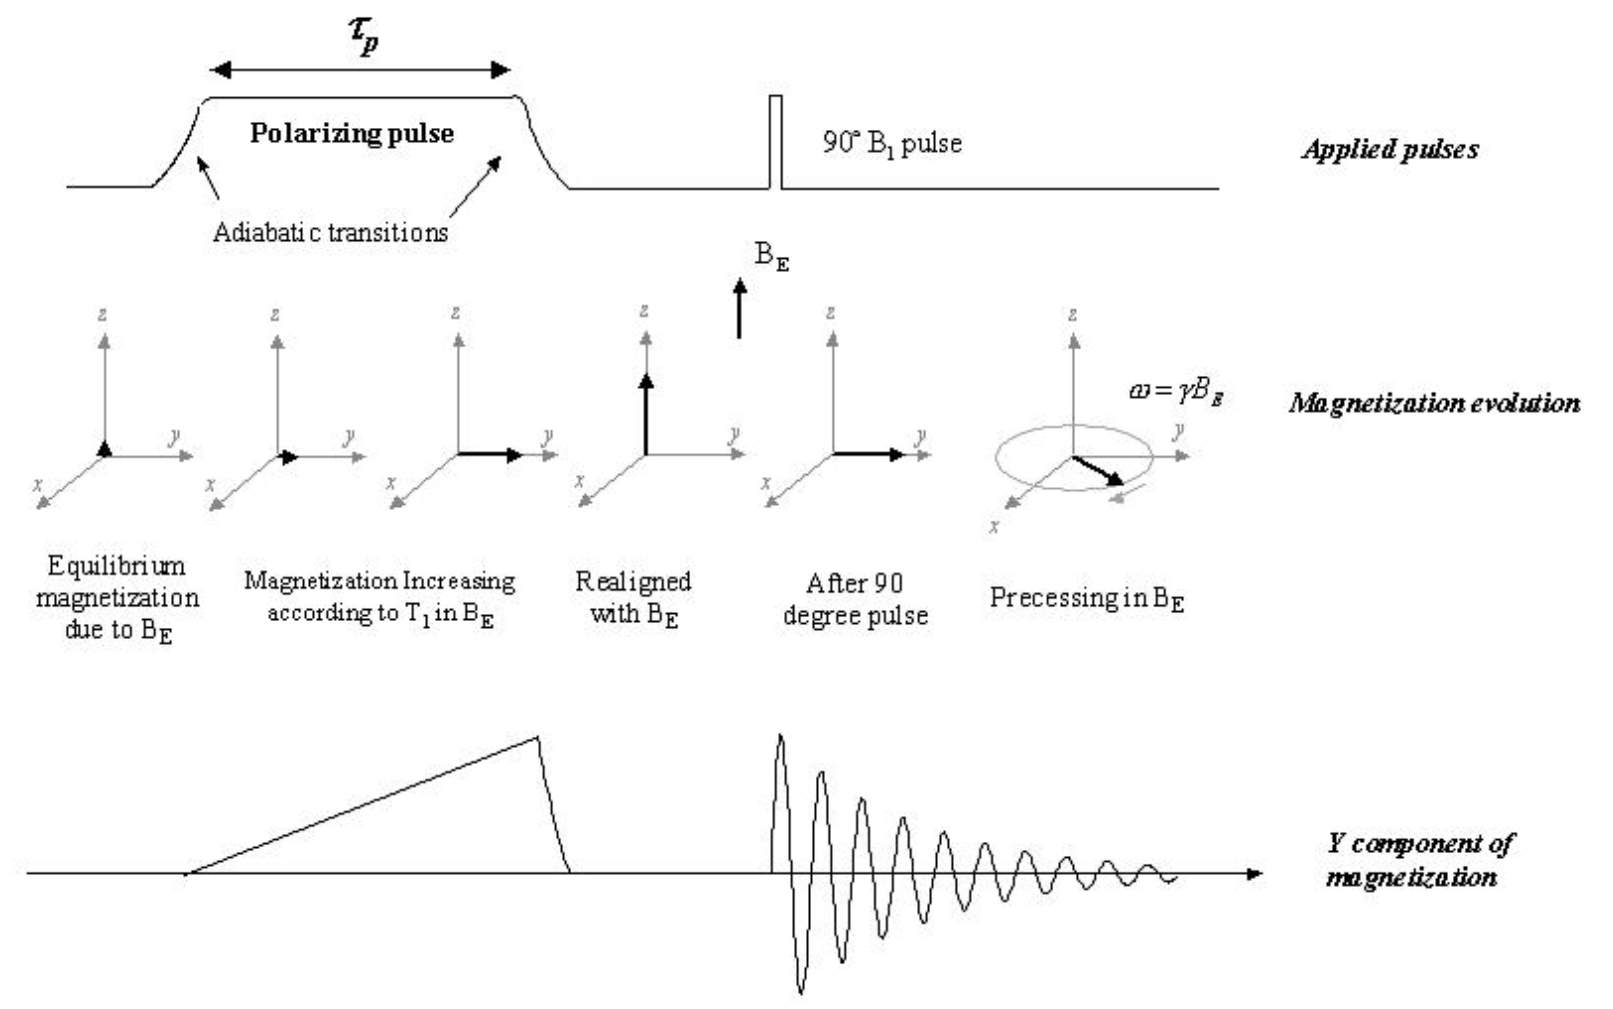
\includegraphics[width=11cm]{../Bilddateien/8/Messprozess.png}
        \caption{Technisches Vorgehen zur Messung der $T_1$ Relaxationszeit.}
        \label{fig:8:Messprozess}
    \end{figure}

    \begin{figure}
        \centering
        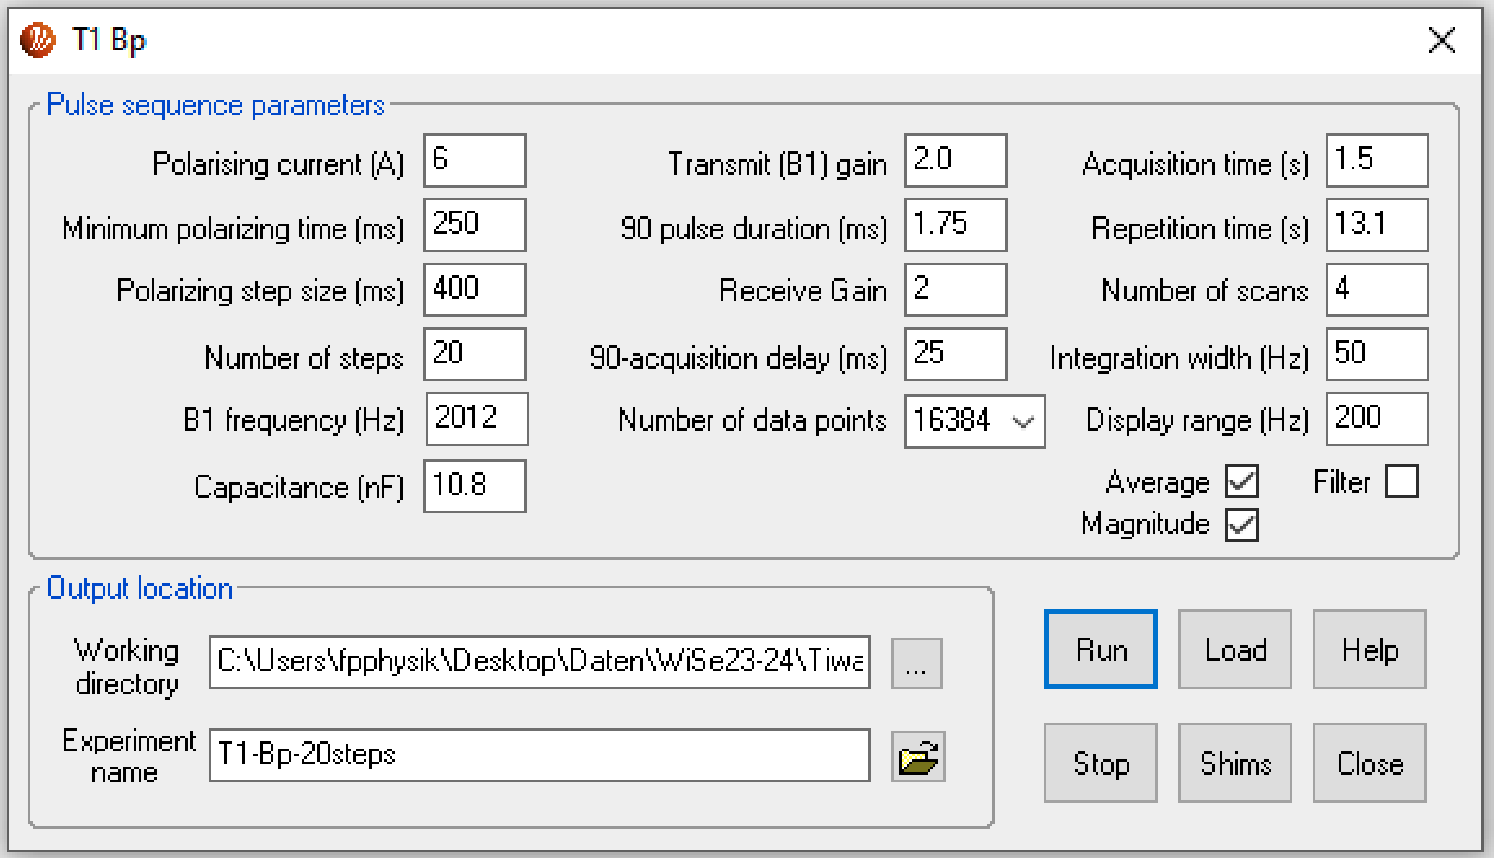
\includegraphics[width=7cm]{../Bilddateien/8/Parameter.png}
        \caption{Ausgewählte Parameter zur Messung der $T_1$ Relaxationszeit.}
        \label{fig:8:Parameter}
    \end{figure}

    Eine Kurvenanpassung führen wir gemäß der Anleitungsformel mithilfe der Funktion 
    \[
        f(x,a,b,c) := 1 - \nbra{a\cdot\exp(-\frac{x}{b}) + c}
    \]
    durch. Dabei schlägt die Anleitung noch eine Skalierung mit der Grundmagnetisierung im Equillibrium $S_0$ vor, welche jedoch durch Normierung $f = S/S_0$ auf $1$ entfällt. Die Fittingkonstante $a$ stellt sich mit $a = 0.986179(3117)$ ebenfalls als nahezu $1$ heraus. Gleiches gilt für $c = -0.00597044$ mit einem relativ zum Wert großen Fehler $u(c) = 0.02279$ ($u(c)/c = 381.7\si{\percent}$), welche wir auf $0$ setzen. Damit erhalten wir dann als $T_1$ Zeit den in der Tabelle \ref{tab:8:T1} aufgeführten Wert. Die Unsicherheit $u(T_1)$ erhalten wir durch die asymptotische Standardabweichung der Kurvenanpassung. 

    \begin{table}[H]
        \centering
        \begin{tabular}{c|cc}
            \hline
            $T_1$ in $\si{\ms}$ & $u(T_1)$ in $\si{\ms}$ & $u(T_1)/T_1$ in $\si{\percent}$ \\
            \hline\hline
            $2268.41$ & $199.9$ & $8.81$ \\
            \hline
        \end{tabular}
        \caption{Ergebnisse zur $T_1$ Relaxationszeit.}
        \label{tab:8:T1}
    \end{table}
    Grafisch haben wir insgesamt zu Beginn eine sehr gute Übereinstimmung zwischen theoretischer Kurvenanpassung und Messwerten, wie in Abbildung \ref{fig:8:T1-Bp-20steps_exp} zu sehen ist. Jedoch ist die Anpassung in den mittleren Messpunkten deutlicher abweichend. Entscheidend ist hier ein Speicherfehler in den Messdaten, welche uns zum Zeitpunkt der Auswertung mit Fehlerintervallradien gleich Null vorliegen. Eine Schätzung der Unsicherheiten der einzelnen Messwerte ist hier also zu ungenau, wir empfehlen eine erneute Messung. Da die Kurvenanpassung jedoch parameterweise Unsicherheiten berechnet, ist die Unkenntnis der Messwertfehler jedoch zu verkraften.
    \begin{figure}[H]
        \centering
        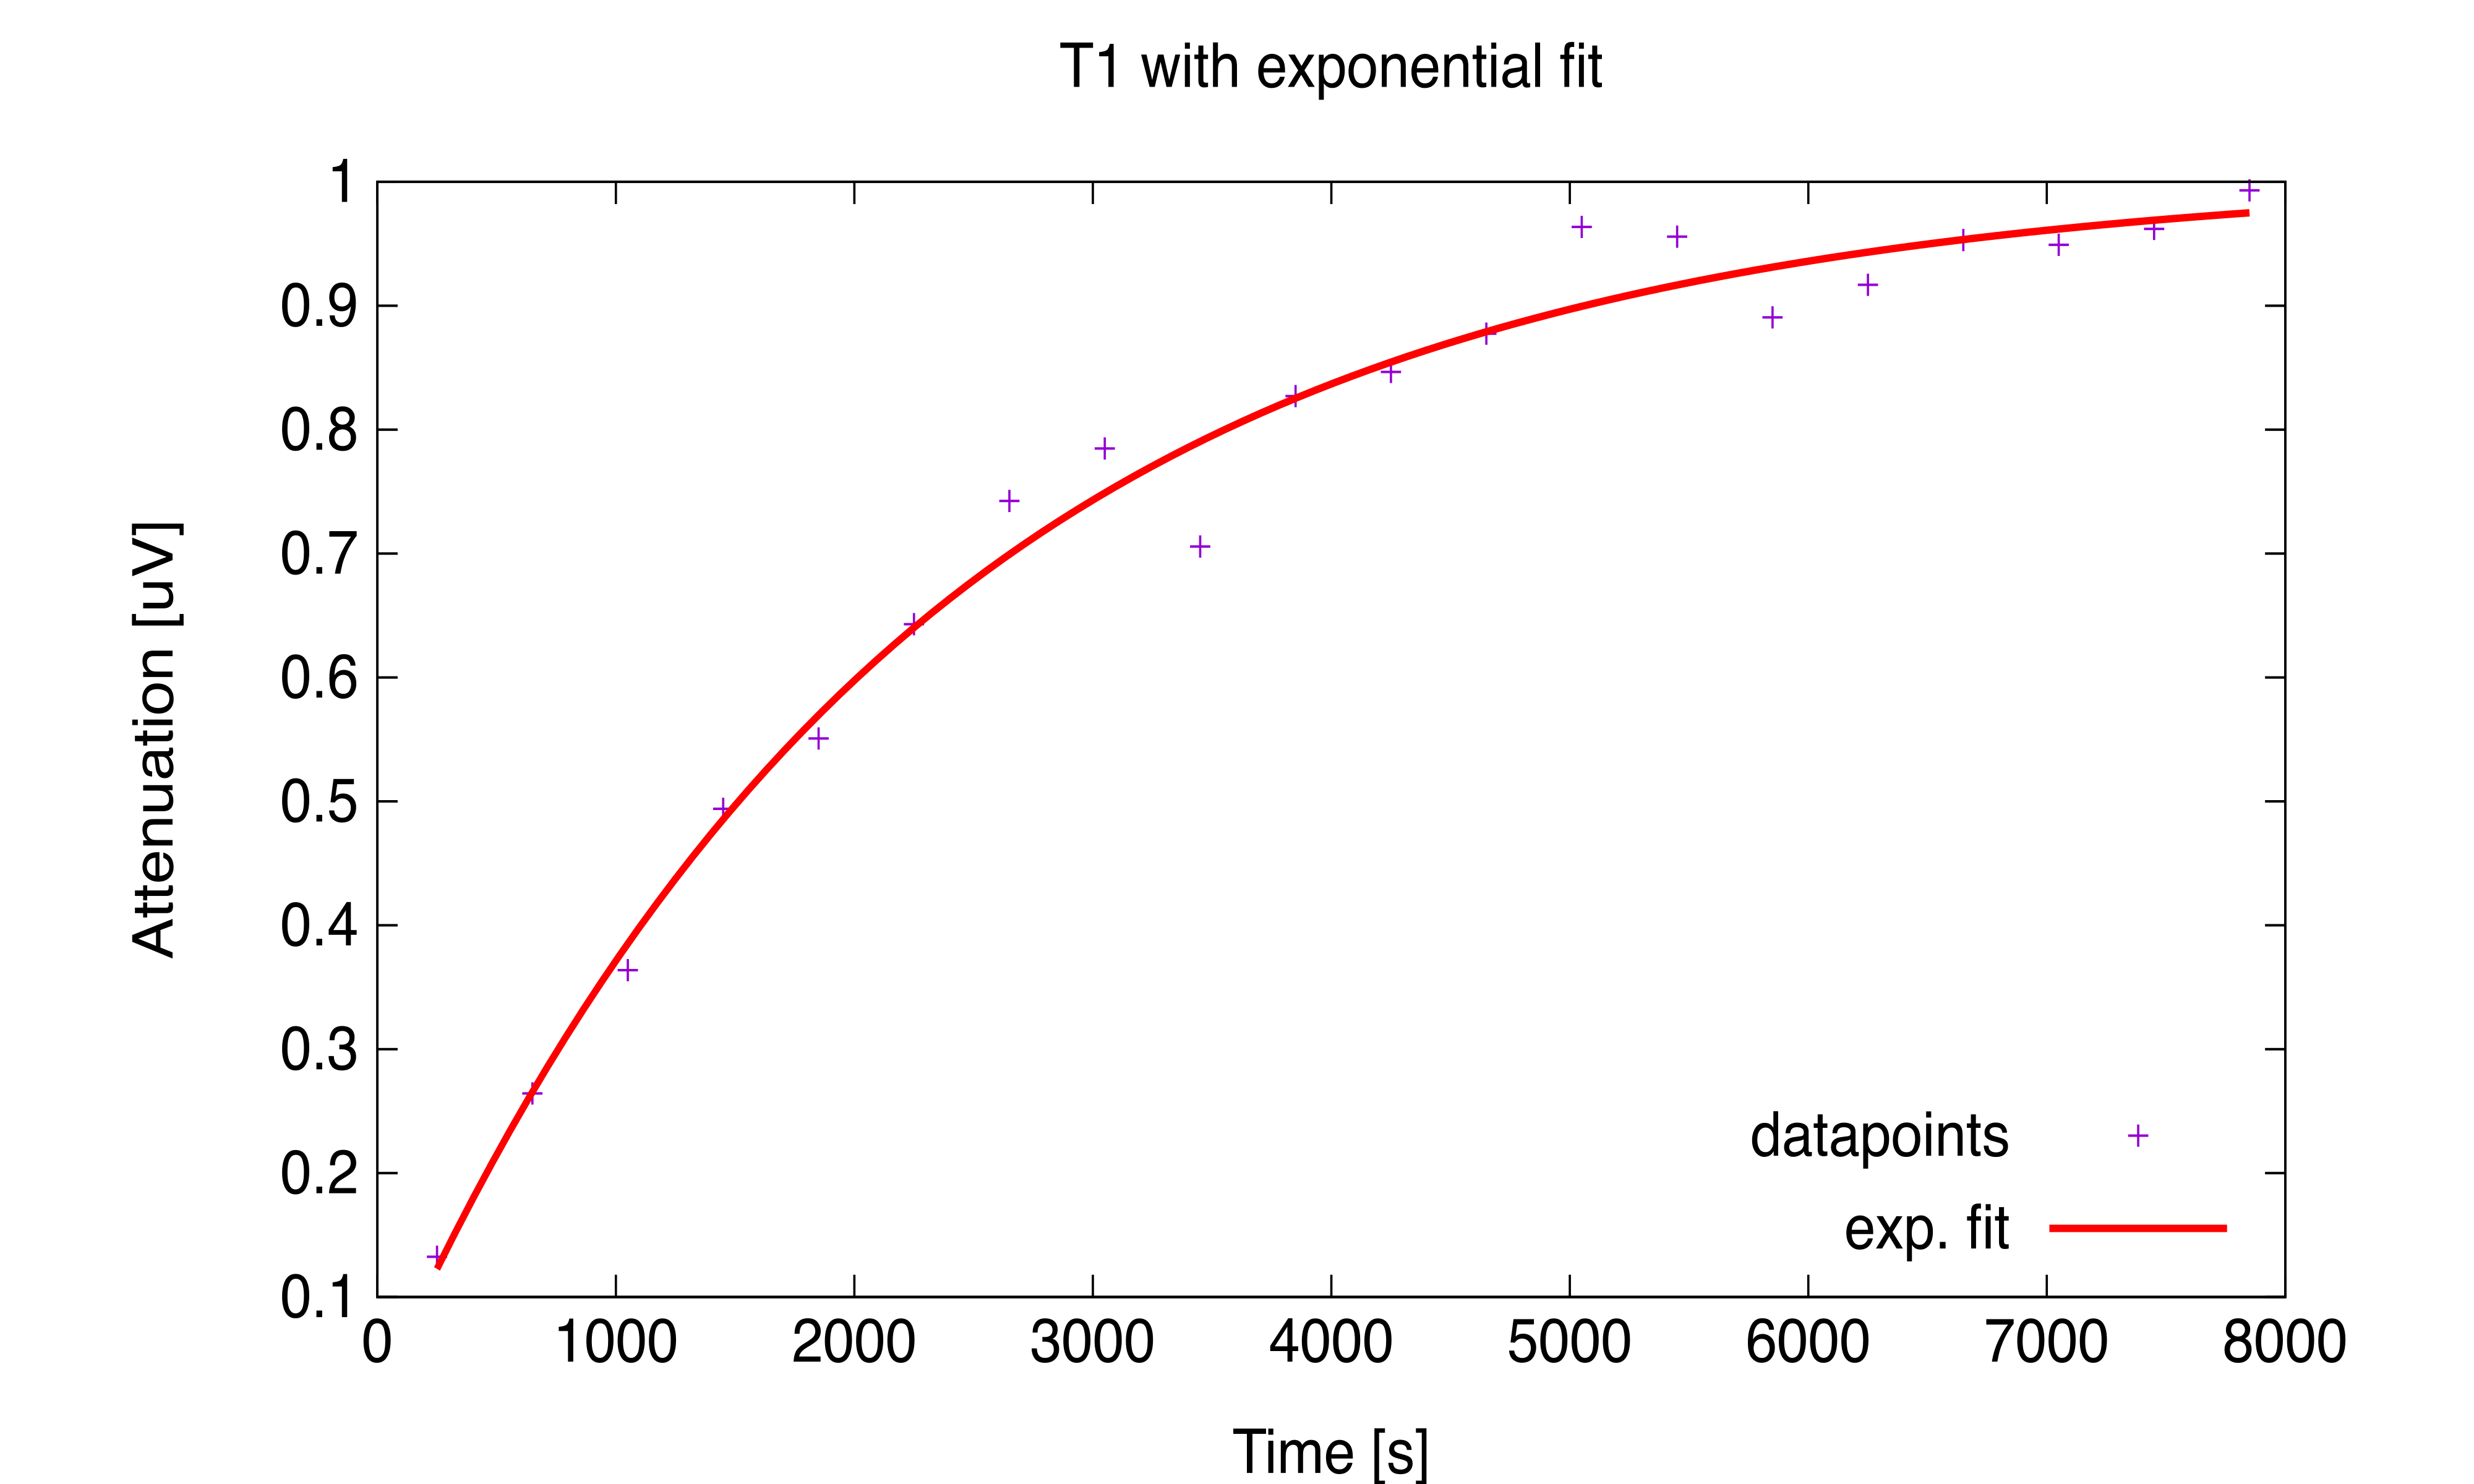
\includegraphics[width=11cm]{../Bilddateien/8/T1-Bp-20steps_exp.png}
        \caption{Messung der $T_1$ Relaxationszeit mit $20$ Messpunkten.}
        \label{fig:8:T1-Bp-20steps_exp}
    \end{figure}
    Die physikalische Interpretation des Graphen ergibt sich durch die $y$ Achsenbeschriftung des Verhältnisses $S(t)/S_0$ (vgl. Wahl $f$). Dieses konvergiert für große $t$ offensichtlich und nach Funktionsdefinition gegen $1$, sodaß wir $T_1$ als Argument der beschreibenden Exponentialfunktion als Parameter der Magnetisierungslebensdauer identifizieren können. 
\end{document}